\synctex=1

\documentclass{article}
\usepackage[utf8]{inputenc}




%%%%%%%%%%%%%%%%%%%%%%%%%%%%%%%%%%%%%%%%%%%%%%%%%%%%%
%%%%%%%%%%%%%%%%%%%%%%%%%%%%%%%%%%%%%%%%%%%%%%%%%%%%%
%%%%% Packages

\usepackage[utf8]{inputenc}
\usepackage[T1]{fontenc}
\usepackage{mathtools}
\usepackage{amssymb}
\usepackage{amsthm}
\usepackage{xspace}
\usepackage{float}
\usepackage{pgf}
\usepackage{tikz}
\usetikzlibrary{backgrounds,arrows,automata,positioning,calc,shadows,fit, patterns}
\usetikzlibrary{shapes.geometric}
\usepackage{array}
\usepackage{booktabs}
\usepackage{changepage}
\usepackage{hyperref}
\usepackage{enumitem}

%%%%%%%%%%%%%%%%%%%%%%%%%%%%%%%%%%%%%%%%%%%%%%%%%%%%%
%%%%%%%%%%%%%%%%%%%%%%%%%%%%%%%%%%%%%%%%%%%%%%%%%%%%%
%%%%% Environments

\newtheorem{theorem}{Theorem}[section]
\newtheorem{lemma}[theorem]{Lemma}
\newtheorem{corollary}[theorem]{Corollary}
\newtheorem{proposition}[theorem]{Proposition}
\newtheorem{claim}[theorem]{Claim}
\newtheorem*{metaproblem}{Meta Problem}
\newtheorem{realproblem}[theorem]{Problem}
\newtheorem{fact}[theorem]{Fact}

\newenvironment{proofsketch}{\noindent\emph{Proof sketch.}}{\hfill$\square$}

\theoremstyle{definition}
\newtheorem{definition}{Definition}
\newtheorem{remark}{Remark}
\newtheorem{example}{Example}

%%%%%%%%%%%%%%%%%%%%%%%%%%%%%%%%%%%%%%%%%%%%%%%%%%%%%
%%%%%%%%%%%%%%%%%%%%%%%%%%%%%%%%%%%%%%%%%%%%%%%%%%%%%
%%%%% Misc. Math

\newcommand{\cceq}{\mathop{::=}}
\newcommand{\myeq}[1]{\stackrel{\text{#1}}{\Leftrightarrow}}

%%%%%%%%%%%%%%%%%%%%%%%%%%%%%%%%%%%%%%%%%%%%%%%%%%%%%
%%%%%%%%%%%%%%%%%%%%%%%%%%%%%%%%%%%%%%%%%%%%%%%%%%%%%
%%%%% Greek Letters
\renewcommand{\epsilon}{\varepsilon}
\renewcommand{\phi}{\varphi}

%%%%%%%%%%%%%%%%%%%%%%%%%%%%%%%%%%%%%%%%%%%%%%%%%%%%%
%%%%%%%%%%%%%%%%%%%%%%%%%%%%%%%%%%%%%%%%%%%%%%%%%%%%%
%%%%% Basic Math

\newcommand{\pow}[1]{2^{#1}}
\newcommand{\nats}{\mathbb{N}}
\newcommand{\size}[1]{|#1|}
\newcommand{\set}[1]{\{ #1 \}}
\newcommand{\ap}[0]{\mathrm{AP}}
\newcommand{\subword}{\preceq}
\newcommand{\nsubword}{\npreceq}
\newcommand{\popartitions}[1]{\mathcal{POP}(#1)}

%%%%%%%%%%%%%%%%%%%%%%%%%%%%%%%%%%%%%%%%%%%%%%%%%%%%%
%%%%%%%%%%%%%%%%%%%%%%%%%%%%%%%%%%%%%%%%%%%%%%%%%%%%%
%%%%% LTL operators

\newcommand{\true}{\mathbf{tt}}
\newcommand{\false}{\mathbf{ff}}
\newcommand{\F}{{\mathbf{F\,}}}
\newcommand{\G}{{\mathbf{G\,}}}
\newcommand{\U}{{\mathbf{\,U\,}}}
\newcommand{\X}{{\mathbf{X\,}}}
\newcommand{\R}{{\mathbf{\,R\,}}}
\newcommand{\Exists}{{\mathbf{E\,}}}
\newcommand{\All}{{\mathbf{A\,}}}


%%%%%%%%%%%%%%%%%%%%%%%%%%%%%%%%%%%%%%%%%%%%%%%%%%%%%
%%%%%%%%%%%%%%%%%%%%%%%%%%%%%%%%%%%%%%%%%%%%%%%%%%%%%
%%%%% Abbrev. for Logics

\newcommand{\ltl}{{LTL}\xspace}
\newcommand{\ctl}{{CTL}\xspace}
\newcommand{\ctlstar}{{CTL$^*$}\xspace}
\newcommand{\fol}{{FO}$[<]$\xspace}
\newcommand{\fole}{{FO}$[<,\,E]$\xspace}
\newcommand{\logics}{$\Lambda$}
\newcommand{\hylogics}{Hyper$\Lambda$\xspace}
\newcommand{\msol}{{MSO}$[<]$\xspace}


\newcommand{\suffix}[2]{#1^{\geq #2}}
\newcommand{\prefix}[2]{#1^{\leq #2}}
\newcommand{\var}{\mathcal{V}}
\newcommand{\eqpoint}[1]{=_{#1}}
\newcommand{\subtree}[2]{#1_{\downarrow #2}}

%%%%%%%%%%%%%%%%%%%%%%%%%%%%%%%%%%%%%%%%%%%%%%%%%%%%%
%%%%%%%%%%%%%%%%%%%%%%%%%%%%%%%%%%%%%%%%%%%%%%%%%%%%%
%%%%% Trace names

\newcommand{\pit}{\pi\text{-trace}}
\newcommand{\taut}{\tau\text{-trace}}
\newcommand{\pits}{\pi\text{-traces}}
\newcommand{\tauts}{\tau\text{-traces}}

%%%%%%%%%%%%%%%%%%%%%%%%%%%%%%%%%%%%%%%%%%%%%%%%%%%%%
%%%%%%%%%%%%%%%%%%%%%%%%%%%%%%%%%%%%%%%%%%%%%%%%%%%%%
%%%%% Complexity

\newcommand{\poly}{\textsc{P}\xspace}
\newcommand{\np}{\textsc{NP}\xspace}
\newcommand{\conp}{\textsc{coNP}\xspace}
\newcommand{\sigmatwo}{$\Sigma_2^{\textsc{P}}$\xspace}
\newcommand{\pitwo}{$\Pi_2^{\textsc{P}}$\xspace}
\newcommand{\sigmathree}{$\Sigma_3^{\textsc{P}}$\xspace}
\newcommand{\pspace}{\textsc{PSpace}\xspace}
\newcommand{\expt}{\textsc{ExpTime}\xspace}
\newcommand{\nexpt}{\textsc{NExpTime}\xspace}
\newcommand{\exps}{\textsc{ExpSpace}\xspace}
\newcommand{\twoexpt}{\textsc{2ExpTime}\xspace}
\newcommand{\tower}{\textsc{Tower}\xspace}

%%%%%%%%%%%%%%%%%%%%%%%%%%%%%%%%%%%%%%%%%%%%%%%%%%%%%
%%%%%%%%%%%%%%%%%%%%%%%%%%%%%%%%%%%%%%%%%%%%%%%%%%%%%
%%%%% Trees
\newcommand{\aut}{\mathcal{A}}
\newcommand{\lang}[1]{\mathcal{L}(#1)}
\newcommand{\initmark}{I}
\newcommand{\kripke}{\mathcal{K}}
\newcommand{\src}[1]{src(#1)}
\newcommand{\tgt}[1]{tgt(#1)}
\newcommand{\runs}[1]{\mathcal{R}(#1)}
\newcommand{\traces}[1]{\mathcal{L}(#1)}
\newcommand{\trace}[1]{tr(#1)}
\newcommand{\game}{\mathcal{G}}
\newcommand{\val}[2]{val_{#1,#2}}
\newcommand{\valstrat}[3]{val^{#2,#3}_{#1}}
\newcommand{\trees}[1]{\mathcal{T}(#1)}
\newcommand{\subformulas}[1]{{Sub(#1)}}
\newcommand{\sons}[2]{Sons_{#2}(#1)}
\newcommand{\treeroot}[1]{root(#1)}
\newcommand{\ancestor}[1]{\preccurlyeq_{#1}}
\newcommand{\descendant}{\succcurlyeq}

%%%%%%%%%%%%%%%%%%%%%%%%%%%%%%%%%%%%%%%%%%%%%%%%%%%%%
%%%%%%%%%%%%%%%%%%%%%%%%%%%%%%%%%%%%%%%%%%%%%%%%%%%%%
%%%%% Probabilities

\newcommand{\distri}[1]{\mathcal{D}(#1)}
\newcommand{\proba}[1]{\mathbb{P}(#1)}

\newcommand{\corto}[1]{\todo[color=red!30]{\small #1}}
\newcommand{\cortoin}[1]{\todo[color=red!30,inline]{\small #1}}




\title{Two-player population games}
\author{}
\date{}

\begin{document}
	
	\maketitle
	
	\section{Non-stochastic reachability}
	
	We reduce this problem to the one player adversarial population reachability game.
	
	The reduction goes as follows: at the start Adam splits the tokens in two groups, one will be used to play the two-player game, the other will serve as a memory to keep track of whose turn it is in a separate system.
	
	Adam has to put tokens in both groups as otherwise Eve can immediately win by some special action. The second group (the memory) is used to keep track of whose player's turn it is. Adam's actions are chosen by allowing him to send tokens to various states $R_i$. After that Eve chooses an action $r_i$, which will send all tokens of $R_j$ with $i\neq j$ to a state $Reset$, from which they will be sent back to the start. However Eve cannot abuse this power to send all tokens of $\mathcal{A}$ to $Reset$, as she has to eventually send tokens to $Win$. Thus she has to always choose an $r_i$ such that there are tokens in $R_i$.
	
	When all tokens of $G$ are in its winning state, they are sent back to the beginning along with all tokens that were sent to $Reset$ in $\mathcal{A}$, while the remaining tokens in $\mathcal{A}$ are sent to $Win$. 
	
	See Figures \ref{fig-nsreach1} and \ref{fig-nsreach2} for an illustration.
	
	\begin{figure}[h]
		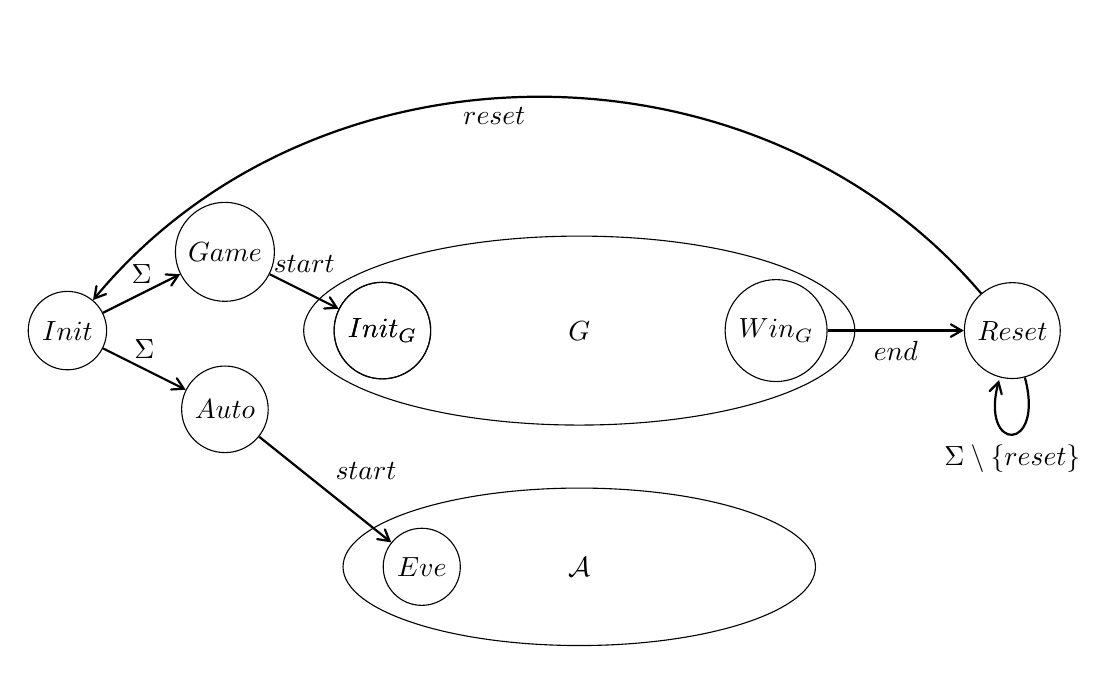
\begin{tikzpicture}
			\node[state] (A) at (-2,0) {$Init$};
			\node[state] (C) at (2, 0) {$Init_G$};
			\node[state] (B) at (10,0) {$Reset$};
			\node[state] (C) at (2, 0) {$Init_G$};
			\node[state] (D) at (7, 0) {$Win_G$};
			\node[state] (H) at (0,1) {$Game$};
			\node[state] (I) at (0,-1) {$Auto$};
			\node (J) at (4.5,0) {$G$};
			\node (J) at (4.5,-3) {$\mathcal{A}$};
			\node[state] (K) at (2.5,-3) {$Eve$};
			
			\draw (4.5,0) ellipse (3.5 and 1.2);
			\draw (4.5,-3) ellipse (3 and 1);
			
			\path[->, thick, >=angle 60] (H) edge node[above=3pt] {$start$} (C);
			\path[->, thick, >=angle 60] (I) edge node[above right] {$start$} (K);
			\path[->, thick, >=angle 60] (A) edge node[above] {$\Sigma$} (H);
			\path[->, thick, >=angle 60] (A) edge node[above] {$\Sigma$} (I);
			\path[->, thick, >=angle 60] (D) edge node[below] {$end$} (B);
			\path[->, thick, >=angle 60, bend right=50] (B) edge node[below left] {$reset$} (A);
			\path[->, thick, >=angle 60, loop below] (B) edge node[below] {$\Sigma\setminus\set{reset}$} (B);
		\end{tikzpicture}
		\caption{Transition system for the non-stochastic reduction}
		\label{fig-nsreach1}
	\end{figure}
	
	\begin{figure}[h]
		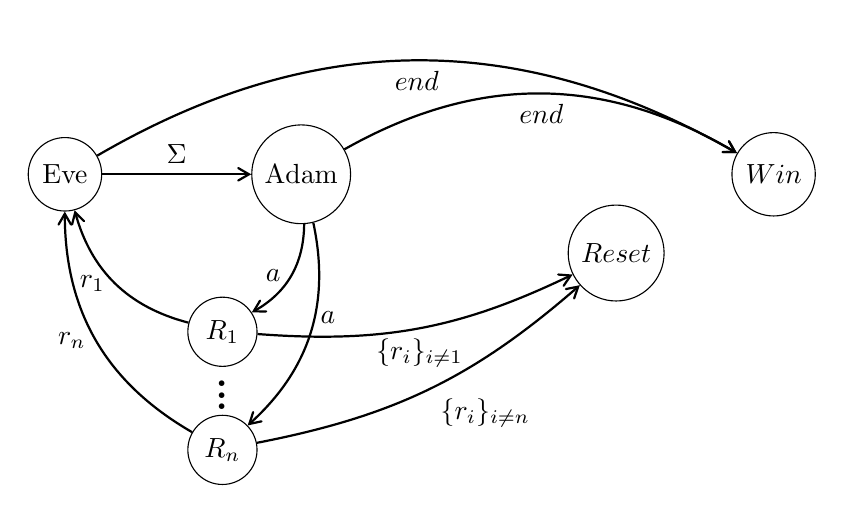
\begin{tikzpicture}
			\node[state] (A) at (0,0) {Eve};
			\node[state] (B) at (3,0) {Adam};
			\node[state] (C) at (2, -2) {$R_1$};
			\node[state] (D) at (2, -3.5) {$R_n$};
			\node (E) at (2,-2.7) {\Huge \vdots};
			\node[state] (F) at (7,-1) {$Reset$};
			\node[state] (G) at (9,0) {$Win$};
			
			
			\path[->, thick, >=angle 60] (A) edge node[above] {$\Sigma$} (B);
			\path[->, thick, >=angle 60, bend left = 30] (B) edge node[left] {$a$} (C);
			\path[->, thick, >=angle 60, bend left = 30] (B) edge node[above right] {$a$} (D);
			\path[->, thick, >=angle 60, bend left = 30] (C) edge node[left] {$r_1$} (A);
			\path[->, thick, >=angle 60, bend left = 30] (D) edge node[left] {$r_n$} (A);
			\path[->, thick, >=angle 60, bend right = 15] (C) edge node[below] {$\set{r_i}_{i \neq 1}$} (F);
			\path[->, thick, >=angle 60, bend right = 15] (D) edge node[below right] {$\set{r_i}_{i \neq n}$} (F);
			\path[->, thick, >=angle 60, bend left = 30] (A) edge node[below] {$end$} (G);
			\path[->, thick, >=angle 60, bend left = 30] (B) edge node[below] {$end$} (G);
			
		\end{tikzpicture}
		\caption{Transition system $\mathcal{A}$ from Figure \ref{fig-nsreach1}}
		\label{fig-nsreach2}
	\end{figure}
	
	
	\section{Stochastic reachability}
	
	We show that the problem of deciding the winner of a two-player stochastic population game is undecidable by reduction from the reachability problem for a two-counter Minsky machine.
	
	Let $\mathcal{M} = (Q, \Delta, init, fin)$ be such a machine, a configuration being an element of $Q \times \nats^2$, with $\Delta \subseteq Q \times \set{++, --, =0?} \times \set{1,2} \times Q$ with the usual semantics.
	
	We describe our construction in several steps: We start with a general map of the system, drawn in Figure~\ref{fig-sreach1}.
	
	\begin{figure}[h]
		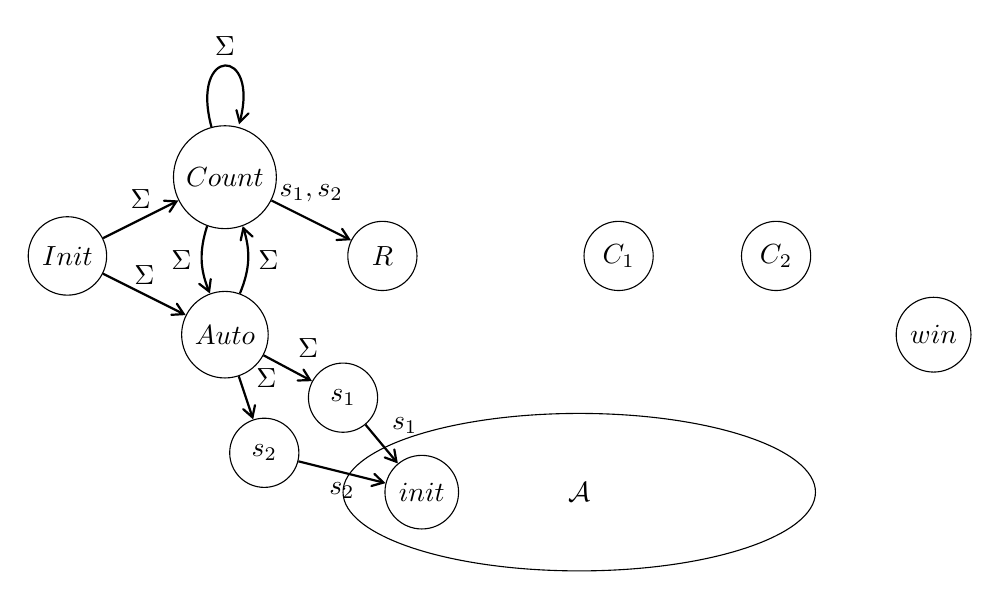
\begin{tikzpicture}
			\node[state] (A) at (-2,0) {$Init$};
			\node[state] (C) at (2, 0) {$R$};
			\node[state] (E) at (5, 0) {$C_1$};
			\node[state] (D) at (7, 0) {$C_2$};
			\node[state] (D) at (9, -1) {$win$};
			\node[state] (H) at (0,1) {$Count$};
			\node[state] (I) at (0,-1) {$Auto$};
			\node (J) at (4.5,-3) {$\mathcal{A}$};
			\node[state] (S1) at (1.5,-1.8) {$s_1$};
			\node[state] (S2) at (0.5,-2.5) {$s_2$};
			\node[state] (K) at (2.5,-3) {$init$};
			
			\draw (4.5,-3) ellipse (3 and 1);
			
			\path[->, thick, >=angle 60, bend right=20] (H) edge node[left] {$\Sigma$} (I);
			\path[->, thick, >=angle 60, bend right=20] (I) edge node[right] {$\Sigma$} (H);
			\path[->, thick, >=angle 60, loop above] (H) edge node[above] {$\Sigma$} (H);
			\path[->, thick, >=angle 60] (H) edge node[above=3pt] {$s_{1}, s_2$} (C);
			\path[->, thick, >=angle 60] (I) edge node[above right] {$\Sigma$} (S1);
			\path[->, thick, >=angle 60] (I) edge node[above right] {$\Sigma$} (S2);
			\path[->, thick, >=angle 60] (S1) edge node[above right] {$s_1$} (K);
			\path[->, thick, >=angle 60] (S2) edge node[below] {$s_2$} (K);
			\path[->, thick, >=angle 60] (A) edge node[above] {$\Sigma$} (H);
			\path[->, thick, >=angle 60] (A) edge node[above] {$\Sigma$} (I);
		\end{tikzpicture}
		\caption{Transition system for the stochastic reduction. There are transitions $reset$ from $s_1$ and $s_2$ to $win$, and from $Count$ and $Auto$ to $Init$}
		\label{fig-sreach1}
	\end{figure}
	
	At the start Eve chooses how to spread tokens between the places $Count$ and $Auto$. 
	However she does not have a real choice: putting more than one token in $Auto$ will give her a positive probability to lose (if tokens go to $s_1$ and $s_2$) while putting no tokens in $Auto$ will allow Adam to reset the game for free.
	
	However if Adam tries to reset the game while Eve did put tokens in Auto, those are sent to the winning state and the game restarts with less tokens, disadvantaging Adam. 
	
	As a result, the players' best choices lead to a configuration where all tokens are in $Count$ except for one which is in $Auto$. We can then start the simulation of $\mathcal{M}$.
	
	The simulation will proceed by rounds, with each round going as follows:
	\begin{itemize}
		\item Adam chooses a transition (and commits to that transition being feasible).
		
		\item Eve executes the associated operation on the counters, and has the opportunity to punish Adam if the chosen transition is not possible.  
	\end{itemize}
	
	If the reserve gets empty then Adam loses. If state $fin$ is reached then Adam wins as it is a sink state. Both players may reset the game to punish each other for cheating. The difference is that Eve will punish Adam by resetting the game while sending some tokens to the winning state, while Adam will punish Eve by sending all tokens (outside the winning state) to the start.
	
	If at any point the reserve $R$ is empty, Eve has an action to send all tokens to $win$ (which also sends tokens of $R$ to $fin$ if it is not empty).
	
	Concretely, there is a place in $\mathcal{A}$ for each state in $Q$ and one for each transition $t \in \Delta$.
	
	From each state Adam will choose an outgoing transition, and the token will stay on the associated place while the operation is checked and executed, after which it will be transferred to the target state of said transition.
	
	For a zero test $=0?$ on counter $C_i$, Eve is allowed to send all tokens (except those of $win$ and $fin$) to the $Start$ state, except those of $C_i$ which are sent to $win$, and those of places of $\mathcal{A}$ not of the form $(q_1, =0?, i, q_2)$ to $fin$.
	
	Hence Eve can only apply that action when Adam chose a transition that tests the emptiness of $C_i$. If $C_i$ was not empty the game restarts with less tokens, advantaging Eve. 
	If $C_i$ was indeed empty, then Eve made no progress.
	
	Thus the best move for Eve is to reset the game that way iff Adam chose a transition of the form $(q_1, =0?, i, q_2)$ and $C_i$ is not empty. 
	
	For an increment $++$ (resp. decrement) on counter $C_i$, Eve chooses a number of tokens to transfer from $R$ to $C_i$ (resp. from $C_i$ to $R$). The mechanism is the same as the one at the start when she chose the number of tokens to send to $Auto$.
	
	If she chooses more than one token she has a positive probability that the tokens split and go to different states, causing her to lose. If she chooses zero, then Adam can reset the game for free (at the condition that the token in $\mathcal{A}$ is indeed in a place of the form $(q_1, ++, i, q_2)$).
	
	If $R$ is empty and the token in $\mathcal{A}$ is in a place of the form $(q_1, ++, i, q_2)$ she can send all tokens to win and win.
	
	Hence Adam has a winning strategy if and only if $fin$ is reachable in $\mathcal{M}$.
	
	\newpage
	
	\section{Safety}
	
	This is much simpler: Say we ignore the tokens and simply play a safety game on the graph. At each state the player who owns it chooses a letter and Adam chooses one of the states accessible by a transition with that letter. If Eve wins then she has an attractor containing the initial state and within the safe area, meaning that she can keep all tokens within that zone and thus win. 
	
	If Adam wins he does so in at most $n$ steps ($n$ being the number of states). In order to win the game with tokens he simply has to put $d^n$ (with $d$ the degree of the graph) tokens in the initial state, allowing him to simulate his strategy in the safety game until he wins without running out of tokens. This holds whether tokens behave in a stochastic or adversarial way, as Eve has to guarantee a winning probability of one.

	

	
\end{document}